\documentclass[EEEE]{KGCOEReport}

\usepackage[backend=biber]{biblatex}
\usepackage{graphicx}
\usepackage{newtxtext, newtxmath}
\usepackage{csquotes}
\usepackage{parskip}
\usepackage{karnaugh-map}
\usepackage{amsmath}
\usepackage{circuitikz}
\usepackage{hyperref}
\usepackage{float}
\usepackage{pdfpages}
\usepackage{pgfplots, pgfplotstable}

\graphicspath{./assets/}
\addbibresource{./assets/bib.bib}

\newcommand{\classCode}{EEEE 281}
\newcommand{\className}{Circuits 1}

\newcommand{\name}{Aden Perry}
% \newcommand{\partnerName}{PARTNER}

\newcommand{\LabSectionNum}{L7}

\newcommand{\TAs}{Sol Holston}
\newcommand{\exerciseNumber}{4}
\newcommand{\exerciseDescription}{Op-amps 1}

\newcommand{\dateDone}{2026-03-14}
\newcommand{\dateSubmitted}{2026-03-21}

\pgfplotsset{compat=1.18}

\begin{document}

\maketitle

\section*{Abstract}


\section{Introduction and Theory}


\subsection{Theory: Circuit Investigated}

Given:

\begin{align*}
	t_{rise}   & = t_{90\%} - t_{10\%}                                  \\
	0.9 V_{in} & = V_(in) \left( 1 - e ^ {-\frac{t_{90\%}}{RC}} \right) \\
	0.1 V_{in} & = V_(in) \left( 1 - e ^ {-\frac{t_{10\%}}{RC}} \right)
\end{align*}

Show:

\begin{equation}
	t_{rise} = t_{90\%} - t_{10\%} = RC \cdot \mathrm{ln}\left(9\right)
\end{equation}

\begin{align*}
	0.9 V_{in}                 & = V_{in} \left( 1 - e ^ {-\frac{t_{90\%}}{RC}} \right)                          \\
	0.9                        & = 1 - e ^ {-\frac{t_{90\%}}{RC}}                                                \\
	e ^ {-\frac{t_{90\%}}{RC}} & = 0.1                                                                           \\
	- \frac{t_{90\%}}{RC}      & = \mathrm{ln}\left(0.1\right)                                                   \\
	-t_{90\%}                  & = RC \cdot \mathrm{ln}\left(0.1\right)                                          \\
	...                                                                                                          \\
	-t_{10\%}                  & = RC \cdot \mathrm{ln}\left(0.9\right)                                          \\
	t_{rise}                   & = - RC \cdot \mathrm{ln}\left(0.1\right) + RC \cdot \mathrm{ln}\left(0.9\right) \\
	t_{rise}                   & = RC \cdot \mathrm{ln}\left(9\right)
\end{align*}

Find capacitive load:

\begin{align*}
	RC \cdot \mathrm{ln}\left(9\right) & < 0.1 \cdot t_{on}                                                                              \\
	C                                  & < \frac{0.1 \cdot t_{on}}{R \cdot \mathrm{ln}\left(9\right)}                                    \\
	C                                  & < \frac{0.1 \cdot \left(\frac{1}{4000}\right)}{\left(50\right) \cdot \mathrm{ln}\left(9\right)} \\
	C                                  & < 0.2275598 \mu \mathrm{F}
\end{align*}

Rounded:

\begin{equation}
	\mathrm{C}_{\text{L,MAX}} = 0.22\text{\mu F}
\end{equation}

\noindent\rule{\linewidth}{0.2pt}

Given:

\begin{align*}
	V_{RIPPLE} & = V_{PEAK} - V_{MIN}                                              \\
	V_{PEAK}   & = \frac{V_{MAX}}{2}                                               \\
	RC         & = - \frac{1}{2f\mathrm{ln}\left(\frac{2 V_{MIN}}{V_{MAX}}\right)} \\
	V_{RIPPLE} & < 0.080
\end{align*}

\begin{align*}
	V_{PEAK} - V_{MIN}          & < 0.08                                                                                     \\
	\frac{V_{MAX}}{2} - V_{MIN} & < 0.08                                                                                     \\
	\frac{3.3}{2} - V_{MIN}     & < 0.08                                                                                     \\
	V_{MIN}                     & < 1.57                                                                                     \\
	(50)C                       & = - \frac{1}{2 \left(2000\right)\mathrm{ln}\left(\frac{2 \left(1.57\right)}{3.3}\right)}   \\
	C                           & = - \frac{1}{100 \left(2000\right)\mathrm{ln}\left(\frac{2 \left(1.57\right)}{3.3}\right)} \\
    C & = 100.604
\end{align*}

Rounded:

\begin{equation}
	\mathrm{C}_{\text{L,MIN}} = 100\text{\mu F}
\end{equation}

\subsection{Theory: LTspice Simulation}


\includegraphics[width=0.8\textwidth]{assets/c1.png}


\includegraphics[width=0.8\textwidth]{assets/c2.png}

Ripple voltage is close to 0.08 V

\section{Hardware Experiment: Results and Discussion}


\includegraphics[width=0.8\textwidth]{assets/c1-hw}

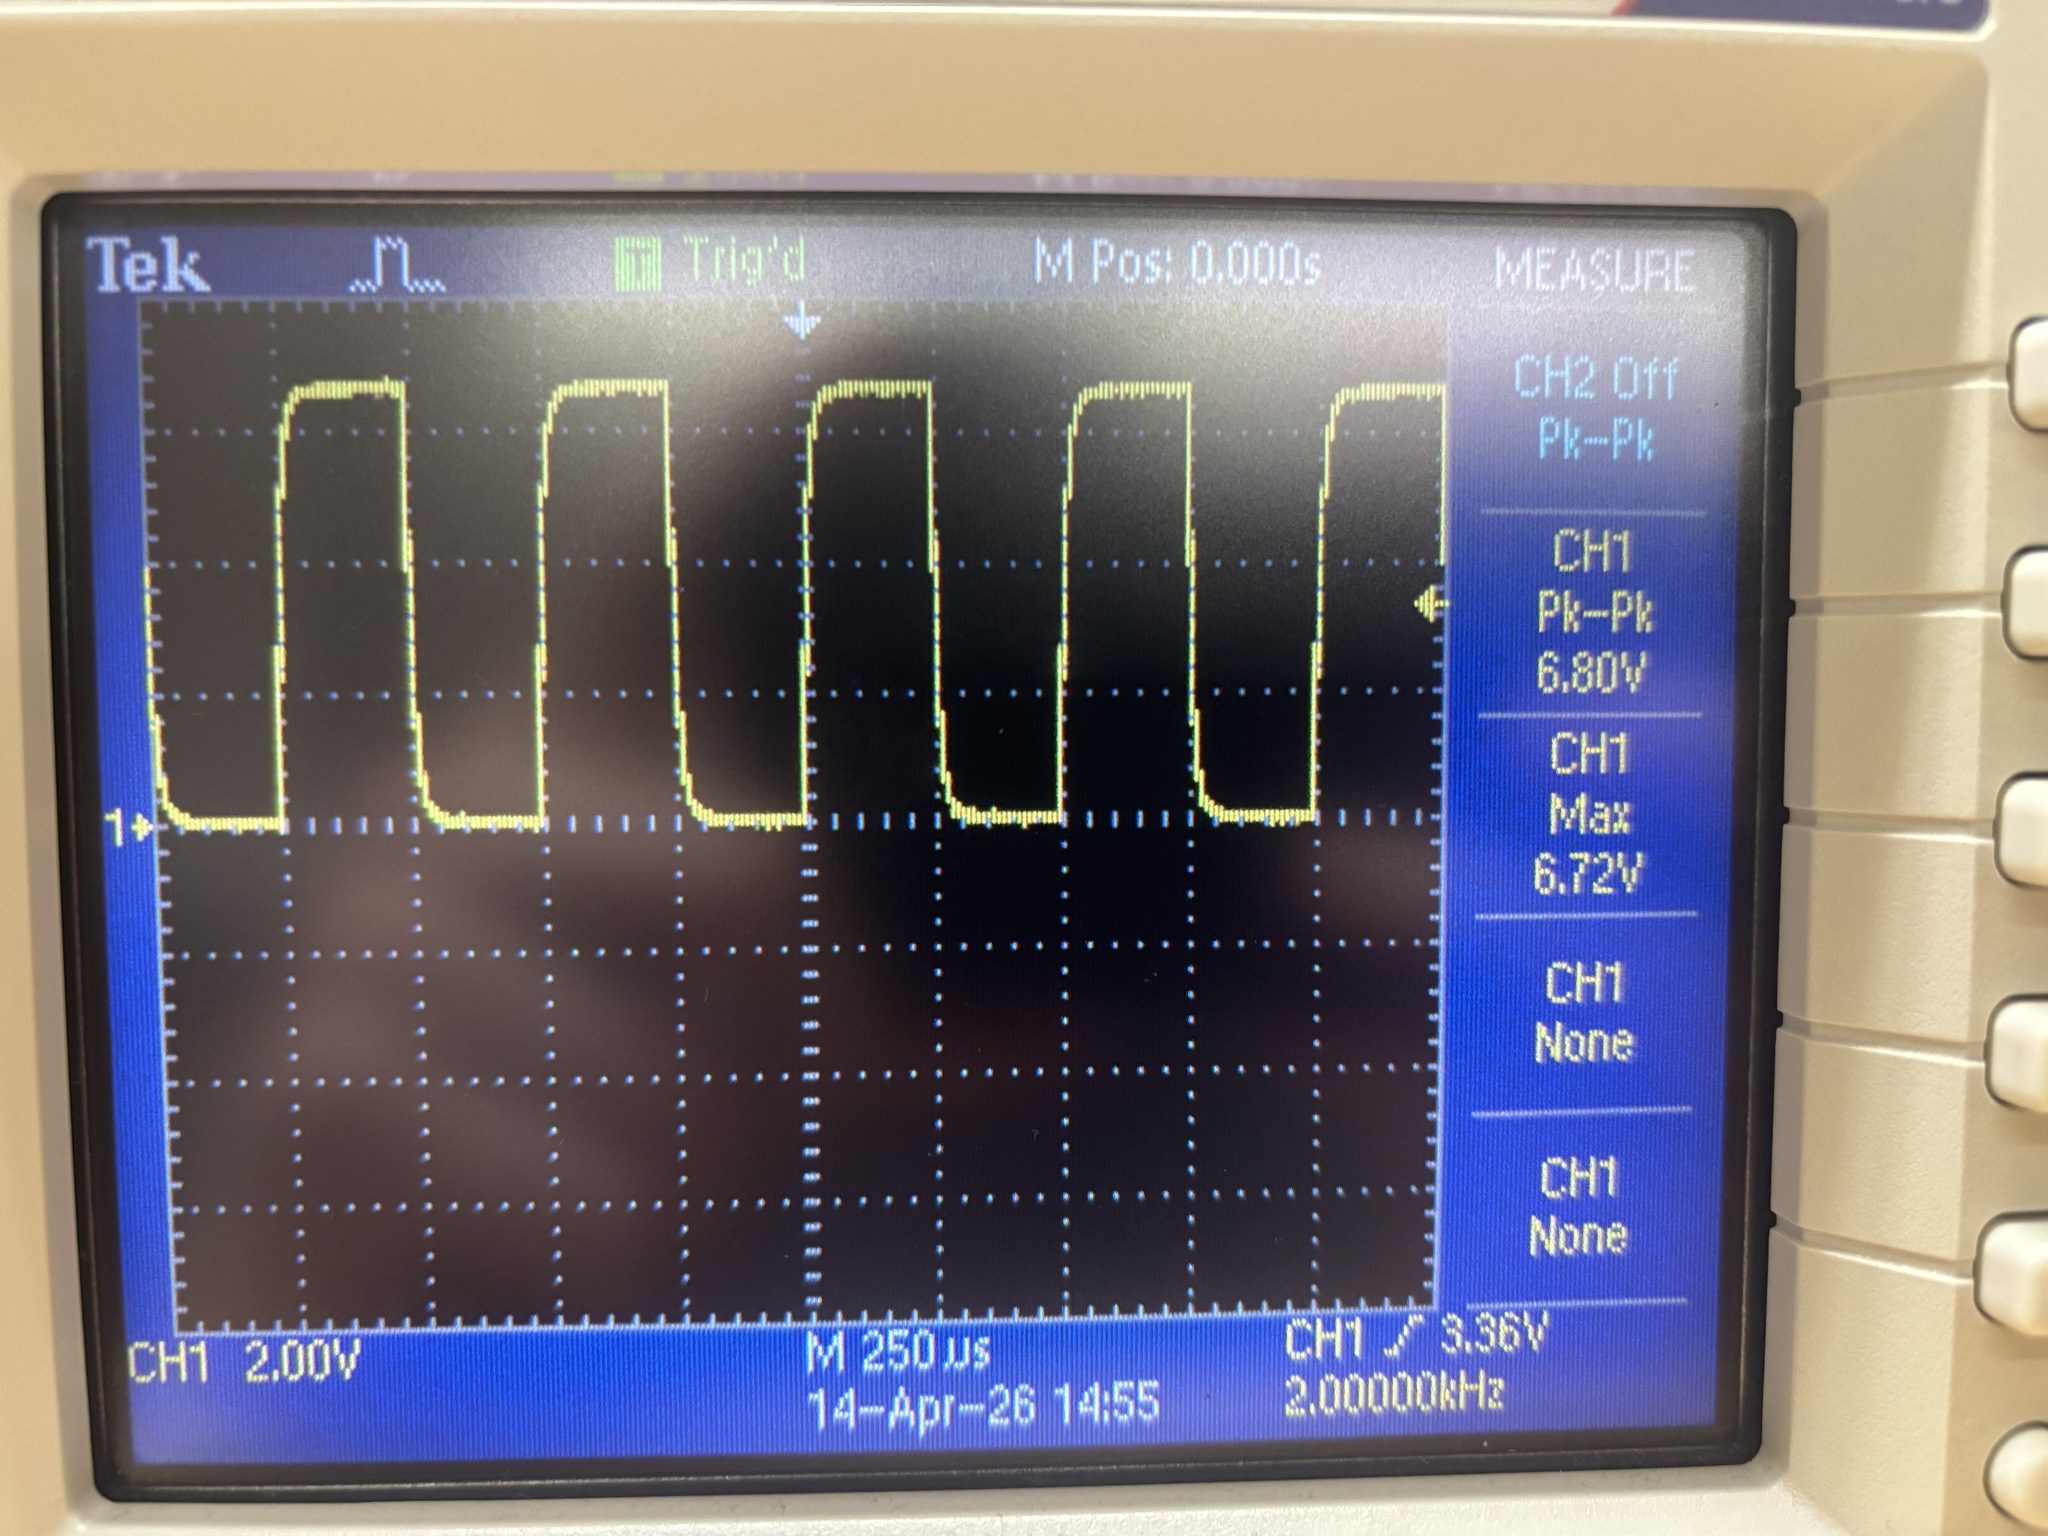
\includegraphics[width=0.8\textwidth]{assets/c1-volt}


\includegraphics[width=0.8\textwidth]{assets/c2-hw}

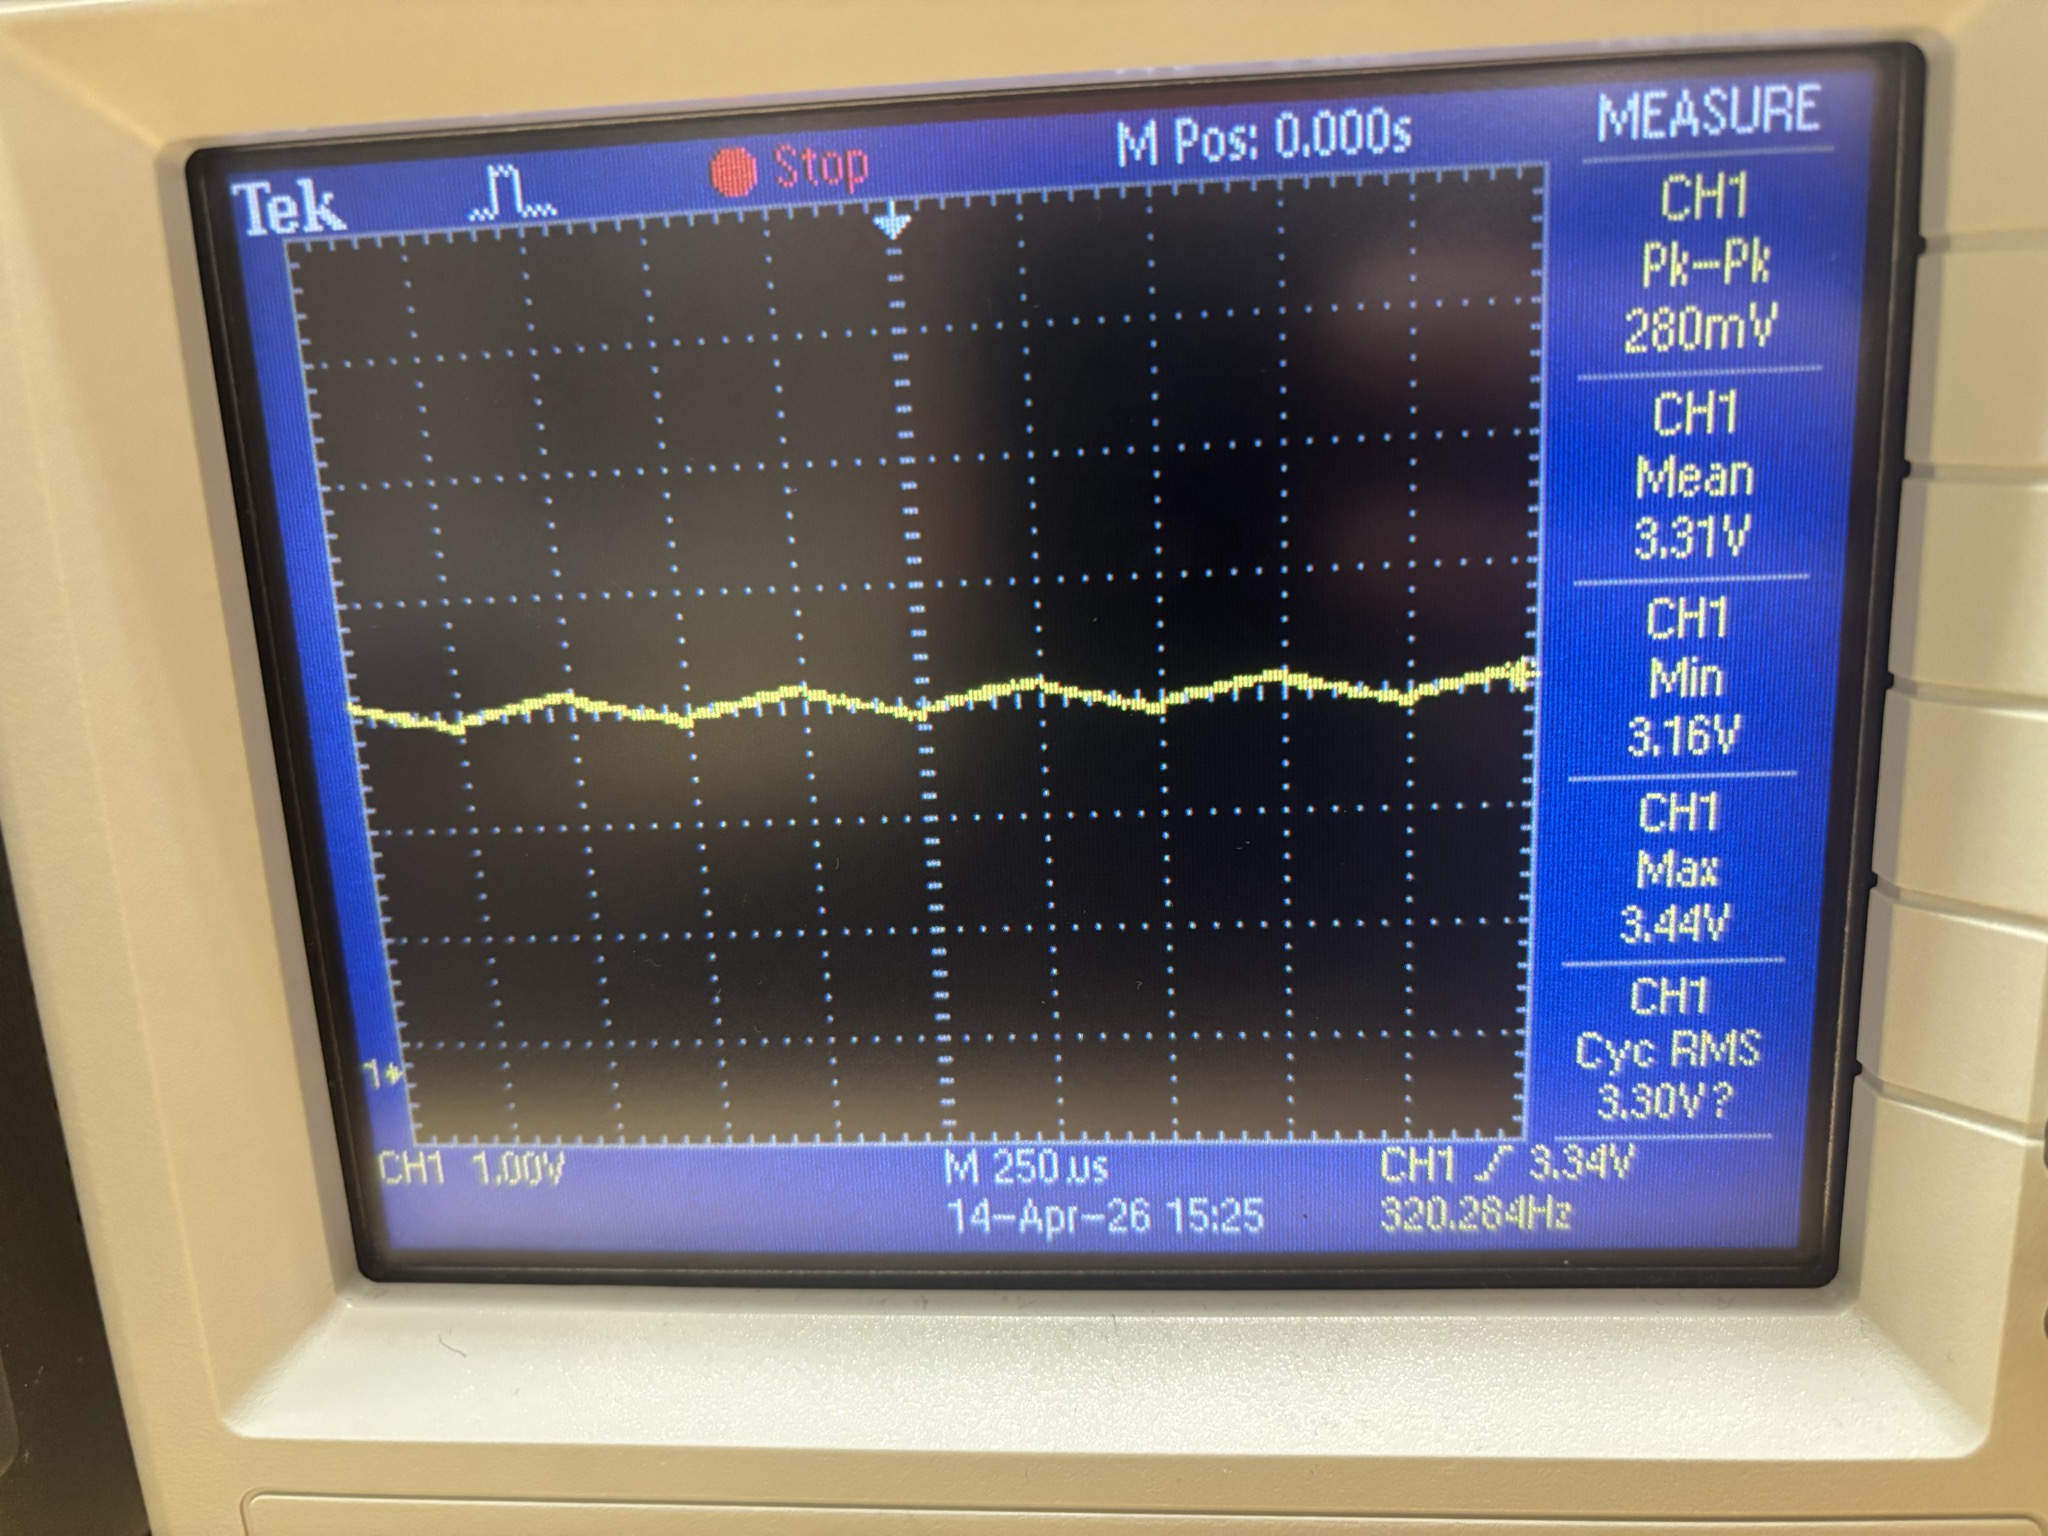
\includegraphics[width=0.8\textwidth]{assets/c2-ripple}

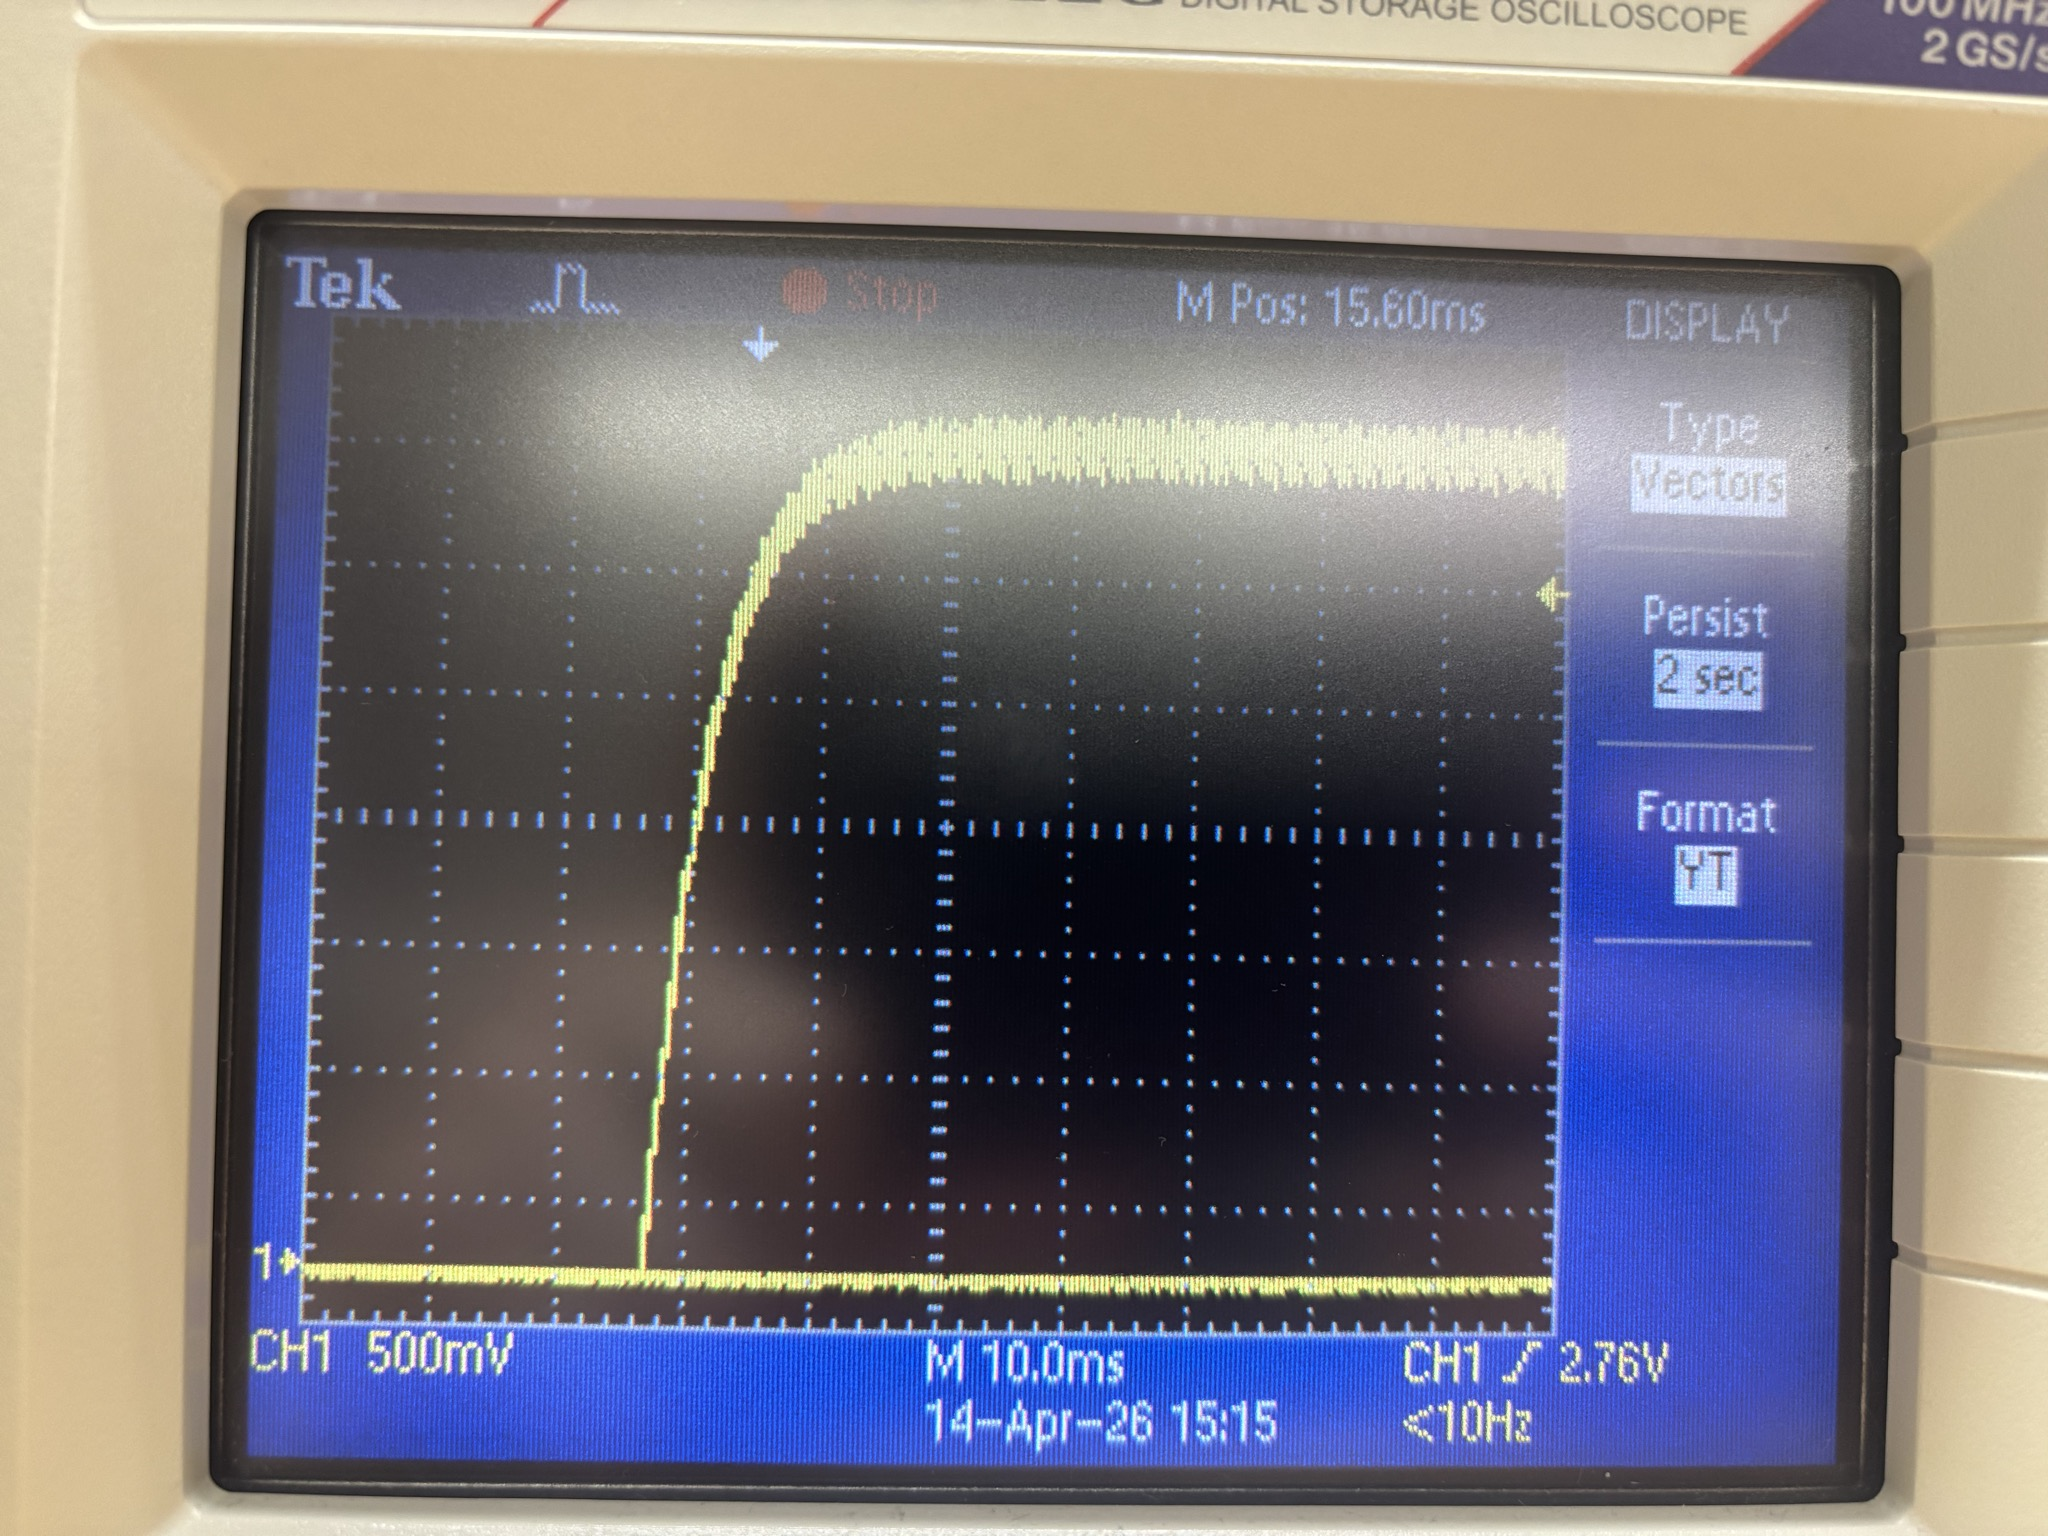
\includegraphics[width=0.8\textwidth]{assets/c2-start}

\section{Conclusion}

Higher capacitive load made the signal more similar to DC, and reduced the
peak-peak voltage.

Hand calcs: 80 mV. Simulation: 80.6 mV. Hardware: 280 mV.

\section{Acknowledgements}

Methods described inthe the textbook \textit{Fundamentals of Electric Circuits,
	7th Edition} \cite{fec} were considered to find Thevenin equivalents.

The template for this Technical Memo was modified from a \LaTeX \ class created
by Joshua Milas and Seth Gower, using the provided Tech Memo Template and
example Tech Memo from the Advanced Course as inspiration.

The Teaching Assistant, Sol Holston, verified that calculated, simulated, and
measured values were correct.

\printbibliography

\end{document}
